\scanpage{22}
\deleted{$A\mathbin{-}A'$}
\deleted{\deleted{$\unsure{A}$}\quad $A'\quad\deleted{T_p(\unsure{A'})}\quad A''\qquad T_p(\unsure{A''_i|A'_i})\simeq T_p(\unsure{A'_i|A''_i})$}
\deleted{\diagram{\begin{tikzcd}[ampersand replacement=\&,column sep=small,row sep=small]S\arrow[r,dash]\&S'\arrow[r,equal]\&S''\\y\arrow[r,dash]\&y'\&y''=y'\amalg y'\end{tikzcd}}}
\deleted{$S-T=T\times_{\unsure{y}}T=T\amalg T$}
\deleted{$T\amalg\uline{T}\amalg\uline{T}$}

\mspage{-0.9-}
then $Y$ is noetherian, or even locally noetherian in all cases (this is an analog of Hilbert's 14th problem). I only know one fact in this direction: if $S=\operatorname{Spec}(k)$, $k$ a field, $X$ is a normal algebraic scheme over $k$, and $(Y,\phi)$ is a \uline{geometric} quotient, then $Y$ is an algebraic scheme over $k$. Since we have no use for this, I omit the proof.
\figure{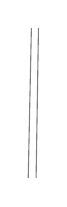
\begin{tikzpicture}\draw[gray](0,0)--(.04,1.9);\draw[gray](.1,0)--(.13,1.9);\end{tikzpicture}}

(3) Suppose $(Y,\phi)$ is a universal categorical quotient. Applying this assumption to the base extensions given by the inclusion of open subsets $U$ in $Y$, one deduces condition (iv) of definition 0.6. More-over, applying it to the inclusion of a single point $y$ in $Y$, and noting that the categorical quotient of an empty scheme by any group is an empty scheme, one deduces that $\phi$ is surjective. Therefore, for $(Y,\phi)$ to be a universal geometric quotient, it is necessary and sufficient that (1) $\phi$ is universally submersive, and (2) the image of $\unsure{\overline{\underline{\psi}}|\overline{\underline{\Psi}}}$ is $X\times_Y X$.

(4) Suppose that the projection from $G$ to $S$ is universally open. This occurs if the projection is flat and of \inserted{loc} finite \figure{\begin{tikzpicture}[baseline=(t.base)]\node[draw,ellipse,inner sep=1pt](t){type};\end{tikzpicture}}, hence for example if $S=\operatorname{Spec}(k)$, $k$ a field, and $G$ is an algebraic group (cf. SGA 4). More generally, this occurs if $S$ is an irreducible normal noetherian pre-scheme, the projection from $G$ to $S$ is \inserted{loc} of finite type, all components of $G$ dominate $S$, and all geometric fibres of $G$ over $S$ have the same dimension: this is Chevalley's
\margin{\unsure{présentation}}
\mspage{21}
